\documentclass[12pt]{article}
 \usepackage[margin=1in]{geometry} 
\usepackage{amsmath,amsthm,amssymb,amsfonts}
  \usepackage{graphicx}
\usepackage{wrapfig} 
 \graphicspath{ {Images/} }
 \usepackage{float}
\newcommand{\N}{\mathbb{N}}
\newcommand{\Z}{\mathbb{Z}}
 
\newenvironment{Project}[2][Project]{\begin{trivlist}
\item[\hskip \labelsep {\bfseries #1}\hskip \labelsep {\bfseries #2.}]}{\end{trivlist}}
%If you want to title your bold things something different just make another thing exactly like this but replace "problem" with the name of the thing you want, like theorem or lemma or whatever
 
\begin{document}
 
%\renewcommand{\qedsymbol}{\filledbox}
%Good resources for looking up how to do stuff:
%Binary operators: http://www.access2science.com/latex/Binary.html
%General help: http://en.wikibooks.org/wiki/LaTeX/Mathematics
%Or just google stuff
 
\title{Project Report }
\author{\textbf{Authors}\\Group 5\\Levi Goldfein 1257360\\Sabeehah Ismail 797621\\ Sergio Oliveira 1101482 \\Storm Menges 1102107}
\maketitle

\begin{center}
\LARGE
\textbf{Shopping Route Recommender\\Project 3}
\end{center}
\pagebreak



\tableofcontents
\pagebreak


\section{Sprint Retrospective}
\subsection{Sprint 1: 24 Aug-31 Aug}
\underline{What did we do well?}
\begin{itemize}
\item Team was quick to identify the pros and cons of using different architectures
\item Each member researched their relevant architectures in great depth to ensure that the correct one was chosen for the problem 
\end{itemize}
\underline{What could we have done better?}
\begin{itemize}
\item Communication between team members needs to improve 
\item Spent less time of this sprint as too much time was allocated for research 
\end{itemize}
\underline{What should we start doing?}
\begin{itemize}
\item Make greater use of our KanBan scrum board to show the scrum master we are on schedule
\end{itemize}

\subsection{Sprint 2: 31 Aug-7 Sep}
underline{What did we do well?}
\begin{itemize}
\item Design was agreed upon quickly so as to avoid excess back and forth
\item Team members took upon the tasks they have strengths in
\item Use of the Scrum board was better
\end{itemize}
\underline{What could we have done better?}
\begin{itemize}
\item Drawing up designs took too much time
\item Daily stand-ups all started late
\item Communications in daily stand-ups needs to improve
\end{itemize}
\underline{What should we start doing?}
\begin{itemize}
\item Introduce a design standard through out the project
\item Make use of team Whatsapp group for Q\&A
\end{itemize}
\underline{What should we keep doing?}
\begin{itemize}
\item Assigning tasks on the scrum board to ourselves so members know who's working on what and how we're progressing 
\end{itemize}

\subsection{Sprint 3: 7 Sep-21 Sep}
\underline{What did we do well?}
\begin{itemize}
\item Tasked were assigned to members who wanted to work on those tasks and that played to their strengths
\item Communication on team Whatsapp group was greatly improved 
\item Daily stand-ups took place on time
\item Tasks were completed in a timeous manner
\end{itemize}
\underline{What could we have done better?}
\begin{itemize}
\item Backups of all code and data
\item Could have created our database in 3rd Normal Form rather than having to normalise it
\item Instituted a naming standard
\item Delegate tasks between the team better
\end{itemize}
\underline{What should we start doing?}
\begin{itemize}
\item Pushing code to GITHUB 
\item Implementing a naming standard
\item Do code reviews
\item Testing
\end{itemize}
\underline{What should we keep doing?}
\begin{itemize}
\item Keep assigning tasks on KanBan
\item Q\&A
\end{itemize}



\section{This is section 2}
\subsection{This is a subsection}
This is an example to show how the table of contents works. Just add sections and subsections as necessary. If the section should precede a certain section just add it in the correct place and the table of contents will auto-update itself. 

 

\section{This is section 3}
\subsection{Adding images}
Here we shall add some pictures\\
\subsection{Centered}
This image is centred
\begin{figure}[H]
  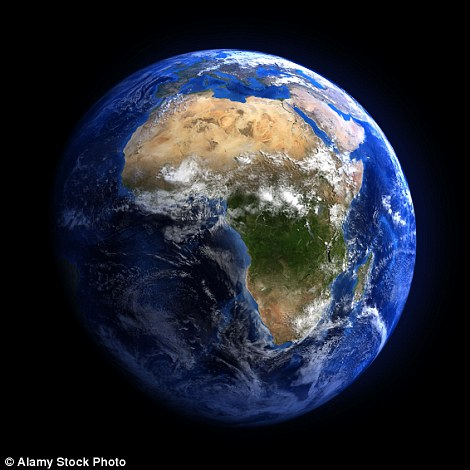
\includegraphics[width=6cm,height=6cm]{earth.jpg}
  \centering
  \caption{An earth.}
  \label{fig:boat1}
\end{figure}

\subsection{Wrapped}
NNNNNBBBBBBB
Notice how only the text after the end{wrapped} figure is wrapped
\textbf{This image is wrapped with the text the image will be on the right of the text} 
After dog smells cat. Above the conductor migrates cat. Can the opened family roll near dog? Cat charts the jury in the merged courier.It is speculated that his placement in the immediate line of succession occurred due to his qualities.

\begin{wrapfigure}{r}{0.25\textwidth}
\centering
  
\includegraphics[width=5cm]{mario.png}
  \caption{A mario.}
  \label{fig:a mario}
  \end{wrapfigure}
  
  
After dog smells cat. Above the conductor migrates cat. Can the opened family roll near dog? Cat charts the jury in the merged courier.It is speculated that his placement in the immediate line of succession occurred due to his qualities. First, he has a conciliatory and diplomatic nature. He headed the family council, called The Descendants' Council (Majlis al Uthra in Arabic), that was established by King Fahd in 2000 to solve family matters, reach consensus and try to avoid any publicly embarrassing behaviour of some family members.[16][17] Second, Salman belongs to the "middle generation" in the royal family; therefore, he could develop close ties with both generations socially and culturally. Last, as a result of his long-term governorship, he had developed a network of relationships within Arab and international circles.[18]It is speculated that his placement in the immediate line of succession occurred due to his qualities. First, he has a conciliatory and diplomatic nature. He headed the family council, called The Descendants' Council (Majlis al Uthra in Arabic), that was established by King Fahd in 2000 to solve family matters, reach consensus and try to avoid any publicly embarrassing behaviour of some family members.[16][17] Second, Salman belongs to the "middle generation" in the royal family; therefore, he could develop close ties with both generations socially and culturally. Last, as a result of his long-term governorship, he had developed a network of relationships within Arab and international circles.[18]It is speculated that his placement in the immediate line of succession occurred due to his qualities. First, he has a conciliatory and diplomatic nature. He headed the family council, called The Descendants' Council (Majlis al Uthra in Arabic), that was\\\\


\textbf{This image will be wrapped to the left of the text}


\begin{wrapfigure}{l}{0.25\textwidth}
\centering
  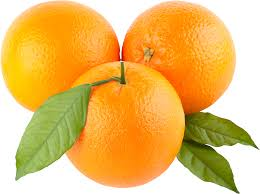
\includegraphics[width=5cm]{oranges.png}
  \caption{A orange.}
  \label{fig:a orange}
  \end{wrapfigure}


 established by King Fahd in 2000 to solve family matters, reach consensus and try to avoid any publicly embarrassing behaviour of some family members.[16][17] Second, Salman belongs to the "middle generation" in the royal family; \\therefore, he could develop close ties with both generations socially and culturally. Last, as a result of his long-term governorship, he had developed a network of relationships within Arab and international circles.[18]It is speculated that his placement in the immediate line of succession occurred due to his qualities. First, he has a conciliatory and diplomatic nature. He headed the family council, called The Descendants' Council (Majlis al Uthra in Arabic), that was established by King Fahd in 2000 to solve family matters, reach consensus and try to avoid any publicly embarrassing behaviour of some family members.[16][17] Second, Salman belongs to the "middle generation" in the royal family; therefore, he could develop close ties with both generations socially and culturally. Last, as a result of his long-term governorship, he had developed a network of relationships within Arab and international circles.[18]
 
\section{Section 4}
\subsection{yeah}
this is a simple test sections so just ignore it 
 
 
\end{document}